\documentclass{standalone}

\usepackage{tikz}
\usetikzlibrary{shapes, arrows}
\usetikzlibrary{arrows,calc,decorations.markings,math,arrows.meta}
\usetikzlibrary{positioning}
\usepackage{graphicx}
\usepackage{adjustbox}




\begin{document}
\trimbox{-0.3cm -0.3cm -0.3cm -0.3cm}{ 
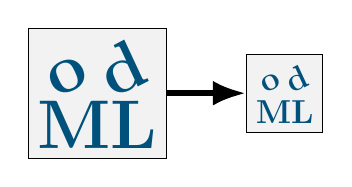
\begin{tikzpicture}

		    \definecolor{odmlcolor}{rgb}{0.00,0.32,0.49}
		    \definecolor{back}{rgb}{0.95,0.95,0.95}
		    \node(odml1) [draw,align=center,font=\bfseries,fill=back]{\Huge \textcolor{odmlcolor}{\rotatebox[origin=c]{25}{o}\rotatebox[origin=c]{25}{d}} \\ \Huge{\textcolor{odmlcolor}{ML}}};
		    
		    \node(odml2) [right=1cm of odml1,draw,align=center,font=\bfseries,fill=back]{\large \textcolor{odmlcolor}{\rotatebox[origin=c]{25}{o}\rotatebox[origin=c]{25}{d}} \\ \large{\textcolor{odmlcolor}{ML}}};
% 		    \node[right = 1cm of odml] (table) {\tikz{
% 		    \begin{scope}[scale=0.35]
% 		      \draw[xstep=1,ystep=0.5] (-2,-2) grid (3,2);
% 		    \end{scope}
% 		    }};
		    
% 		    \node[above = 0cm of table](tabletext) {};
		    
		    \draw[-{Latex[scale=1]},line width=0.7mm] (odml1.east) -- (odml2.west) {};
% 		    \draw[{Latex[scale=1]}-,line width=0.7mm] ([yshift=-0.2cm]odml.east) -- ([yshift=-0.2cm]table.west) {};

	
\end{tikzpicture}
}
\end{document}